% !TeX root = mainstarkov.tex
% !TeX program = xelatex
% !TeX encoding = UTF-8
\section{Техническое задание}

\subsection{Основание для разработки}

Основанием для разработки является задание на выпускную квалификационную работу по теме «\Тема\ \ТемаВтораяСтрока\ \ТемаТретьяСтрока». Разработка ведётся в соответствии с ГОСТ 19.102-77 \cite{gost19102} (стадии разработки) и ГОСТ 19.201-78 \cite{gost19201} (требования к техническому заданию).

Объектом разработки является алгоритмическое ядро системы построения эвакуационных маршрутов в реальном времени для замкнутых пространств, реализованное в виде модуля динамической маршрутизации приложения IndoorNav.

\subsection{Назначение разработки}

\textbf{Функциональное назначение.} Модуль динамической маршрутизации предназначен для:
\begin{itemize}
\item построения кратчайших маршрутов между точками внутри здания с учётом весов рёбер;
\item поиска ближайшего эвакуационного выхода из текущего положения пользователя;
\item динамического перестроения маршрута при блокировке участков пути;
\item обработки межэтажных переходов;
\item восстановления последовательности узлов маршрута для навигации пользователя.
\end{itemize}

\textbf{Эксплуатационное назначение.} Модуль предназначен для использования в составе кроссплатформенного приложения IndoorNav на мобильных устройствах (Android, iOS) и настольных компьютерах (Windows). В штатном режиме модуль обеспечивает построение маршрутов между помещениями; в режиме ЧС -- автоматическое построение эвакуационного маршрута до ближайшего безопасного выхода.

\subsection{Требования к программной системе}

\subsubsection{Требования к данным программной системы}

Входными данными для модуля маршрутизации являются:
\begin{itemize}
\item навигационный граф в формате JSON (узлы, рёбра, здания, этажи);
\item идентификатор стартового узла (string);
\item идентификатор конечного узла (string);
\item множество исключённых узлов (\texttt{ISet<string>}, может быть пустым);
\item текущее состояние режима ЧС (флаг активности, идентификатор здания).
\end{itemize}

Выходными данными модуля являются:
\begin{itemize}
\item упорядоченный список узлов маршрута от старта до цели (\texttt{List<NavNode>});
\item пустой список при отсутствии пути;
\item суммарный вес маршрута (float);
\item путь до ближайшего эвакуационного выхода при активации ЧС.
\end{itemize}

Концептуальная модель данных модуля включает сущности: навигационный узел (NavNode), навигационное ребро (NavEdge), навигационный граф (NavGraph). Навигационный узел имеет тип (аудитория, коридор, лестница, лифт, выход, запасной выход, QR-якорь) и координаты на плане этажа. Навигационное ребро связывает два узла и имеет вес, вычисляемый как евклидово расстояние или штраф для межэтажных переходов.

\subsubsection{Требования к функциям программной системы}

\paragraph{Построение маршрута между точками.} Модуль должен:
\begin{itemize}
\item строить кратчайший путь между двумя заданными узлами графа по алгоритму Дейкстры;
\item учитывать веса рёбер при вычислении оптимального пути;
\item корректно обрабатывать ситуацию отсутствия пути (несвязный граф, полная блокировка);
\item обеспечивать время выполнения не более 200 мс для графа до 500 узлов и 1000 рёбер;
\item возвращать упорядоченный список узлов маршрута (начало → конец);
\item возвращать пустой список при совпадении стартового и конечного узла (путь из одного элемента);
\item возвращать пустой список при несуществующих идентификаторах узлов.
\end{itemize}

\paragraph{Динамическое исключение узлов.} Алгоритм должен поддерживать:
\begin{itemize}
\item передачу множества исключаемых узлов как параметра без модификации исходного графа;
\item игнорирование исключённых узлов при релаксации рёбер;
\item невозможность исключения конечного узла маршрута (даже если он в множестве);
\item корректную работу при последовательном добавлении исключений (повторный вызов);
\item использование \texttt{HashSet<string>} для проверки принадлежности множеству за $O(1)$;
\item возврат пустого результата при исключении всех возможных путей.
\end{itemize}

\paragraph{Поиск эвакуационного выхода.} Реализация должна обеспечивать:
\begin{itemize}
\item поиск кратчайшего пути до ближайшего узла с флагом \texttt{IsExit} или \texttt{IsEvacuationExit};
\item приоритет выходов в том же здании (\texttt{BuildingId}) при наличии нескольких корпусов;
\item автоматическое построение маршрута при активации режима ЧС;
\item возврат пустого результата при отсутствии доступных выходов;
\item учёт исключённых узлов и заблокированных участков при поиске выхода;
\item выбор выхода с минимальной суммой веса рёбер;
\item fallback на выходы других зданий при отсутствии выходов в текущем.
\end{itemize}

\paragraph{Обработка межэтажных переходов.} Система должна:
\begin{itemize}
\item корректно обрабатывать рёбра, соединяющие узлы разных этажей;
\item учитывать вес ребёр;
\item избегать ненужных смен этажей при наличии прямого горизонтального пути;
\item гарантировать достижимость любого этажа при отсутствии блокировок;
\item различать типы переходов: лестница вверх, лестница вниз, лифт;
\item формировать пошаговые инструкции при смене этажа.
\end{itemize}

\paragraph{Восстановление пути.} Алгоритм должен:
\begin{itemize}
\item сохранять предшественника для каждого достижимого узла;
\item восстанавливать полный путь от старта до цели обратным обходом;
\item возвращать путь в порядке от стартового узла к конечному;
\item корректно обрабатывать случай, когда старт и цель совпадают.
\end{itemize}

\subsubsection{Требования к структурам данных}

\paragraph{Представление графа.} Граф должен храниться в формате, обеспечивающем:
\begin{itemize}
\item быстрый доступ к узлу по идентификатору через словарь (\texttt{Dictionary<string, NavNode>});
\item хранение списка смежности для каждого узла (\texttt{Dictionary<string, List<(string, float)>>});
\item хранение весов рёбер в формате \texttt{float};
\item поддержку неориентированных рёбер (двунаправленных);
\item сериализацию/десериализацию в JSON для загрузки и сохранения.
\end{itemize}

\paragraph{Узлы графа.} Узел (\texttt{NavNode}) должен содержать:
\begin{itemize}
\item уникальный идентификатор (string);
\item координаты на плане этажа (float X, Y);
\item номер этажа (int);
\item идентификатор здания (string);
\item тип узла (обычный, переход, выход, эвакуационный выход, огнетушитель, QR-якорь);
\item отображаемое название (string);
\item необязательный идентификатор помещения;
\item флаги: \texttt{IsTransition}, \texttt{IsElevator}, \texttt{IsExit}, \texttt{IsEvacuationExit}, \texttt{IsQrAnchor};
\item идентификатор группы перехода (\texttt{TransitionGroupId}) для связывания узлов на разных этажах.
\end{itemize}

\paragraph{Рёбра графа.} Ребро (\texttt{NavEdge}) должно содержать:
\begin{itemize}
\item идентификаторы соединяемых узлов (\texttt{FromId}, \texttt{ToId});
\item вес (евклидово расстояние или заданное значение);
\item флаг межэтажного перехода (\texttt{IsCrossFloor}).
\end{itemize}

Вес ребра вычисляется автоматически: для узлов на одном этаже $w = \sqrt{(x_2 - x_1)^2 + (y_2 - y_1)^2}$, для узлов на разных этажах $w = 150$.

\subsubsection{Нефункциональные требования}

\textbf{Требования к производительности.}
\begin{itemize}
\item построение маршрута: не более 200 мс для графа до 500 узлов;
\item поиск ближайшего выхода: не более 300 мс;
\item потребление памяти: не более 50 МБ для графа здания;
\item масштабируемость: поддержка графов до 1000 узлов и 2000 рёбер;
\item построение списка смежности: не более 50 мс при загрузке графа.
\end{itemize}

\textbf{Требования к надёжности.}
\begin{itemize}
\item корректная работа при некорректных входных данных (несуществующие ID узлов);
\item возврат пустого результата вместо исключения при отсутствии пути;
\item устойчивость к циклическим исключениям узлов;
\item обработка граничных случаев: граф из одного узла, старт = конец, петли;
\item сохранение корректности при повторных вызовах с разными параметрами исключений;
\item отсутствие утечек памяти при многократном построении маршрутов.
\end{itemize}

\textbf{Требования к совместимости.}
\begin{itemize}
\item совместимость с .NET 9 и MAUI workload;
\item работа на Android 8.0+, iOS 15+ и Windows 10/11;
\item использование только стандартных коллекций .NET (без нативных зависимостей).
\end{itemize}

\subsection{Сценарии использования}

С системой работают три типа пользователей (актёров):
\begin{itemize}
	\item \textbf{Гость} -- входит без регистрации; ему доступны построение маршрута, поиск ближайшего выхода, блокировка узла и навигация по QR-коду;
	\item \textbf{Студент} -- авторизуется и вдобавок к возможностям гостя получает построение маршрута к аудитории из своего расписания;
	\item \textbf{Администратор} -- размечает карту здания, управляет пользователями и включает режим ЧС по корпусам.
\end{itemize}

Распределение вариантов использования по ролям пользователей представлено на рисунке~\ref{usecase:image}.

\begin{figure}[H]
	\centering
	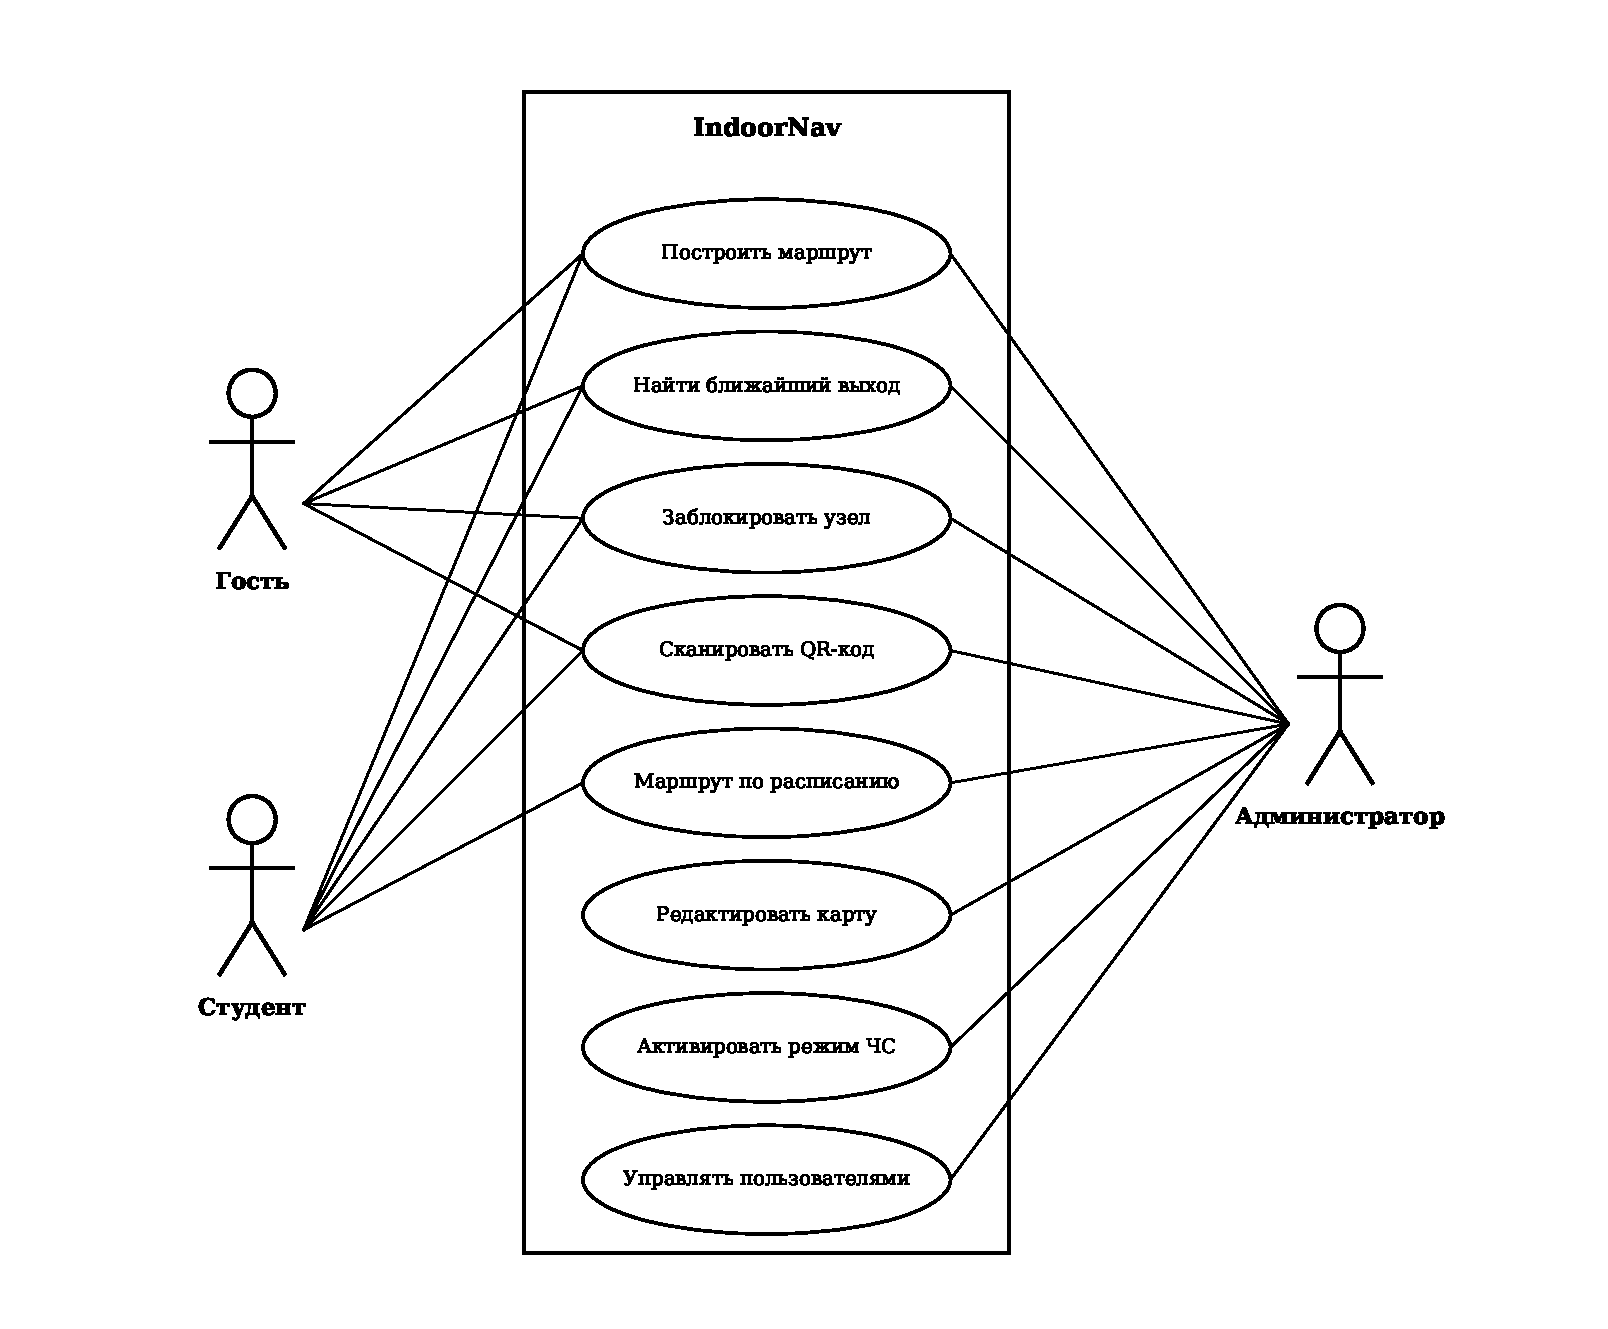
\includegraphics[width=0.95\textwidth]{Pictures/usecase.eps}
	\caption{Диаграмма вариантов использования}
	\label{usecase:image}
\end{figure}

Ниже подробно разобраны три ключевых сценария: построение повседневного маршрута, эвакуация и перестроение маршрута при блокировке.

\subsubsection{Построение маршрута}

Сценарий навигации:
\begin{enumerate}
\item Пользователь выбирает начальную точку (вручную или через QR).
\item Пользователь выбирает конечную точку (поиск по названию или нажатием на карту).
\item ViewModel вызывает метод \texttt{NavGraph.FindPath(startId, endId, excludeIds)}.
\item Алгоритм Дейкстры строит кратчайший путь с учётом исключённых узлов.
\item Маршрут возвращается как упорядоченный список узлов.
\item ViewModel формирует пошаговые инструкции и отображает маршрут на карте.
\end{enumerate}

\subsubsection{Построение эвакуационного маршрута}

Сценарий эвакуации:
\begin{enumerate}
\item Система получает от сервера флаг активации ЧС.
\item ViewModel вызывает метод \texttt{EmergencyService.FindNearestExitRoute(start, graph, blocked)}.
\item Сервис определяет все доступные эвакуационные выходы в текущем здании.
\item Для каждого выхода вычисляется кратчайший путь алгоритмом Дейкстры.
\item Маршрут возвращается как список узлов от текущего положения до выхода.
\item При отсутствии достижимых выходов возвращается пустой список.
\end{enumerate}

\subsubsection{Блокировка участка и перестроение маршрута}

Сценарий обхода препятствия:
\begin{enumerate}
\item Пользователь нажимает на узел и выбирает <<Заблокировать>>.
\item Идентификатор узла добавляется в множество заблокированных (\texttt{HashSet<string>}).
\item ViewModel формирует множество исключений: все выходы (кроме начального и конечного) и заблокированные узлы.
\item Вызывается метод \texttt{FindPath} с обновлённым множеством исключений.
\item Алгоритм строит маршрут в обход заблокированного узла.
\item Если путь отсутствует, то отображается сообщение <<Маршрут не найден>>.
\end{enumerate}

\subsection{Требования к тестированию}

\subsubsection{Объём тестирования}

Разработка должна включать:
\begin{itemize}
\item модульные тесты для алгоритма Дейкстры;
\item модульные тесты для алгоритма поиска ближайшего выхода;
\item тесты производительности (замеры времени выполнения на разных размерах графа);
\item тесты с динамическим исключением узлов (последовательная блокировка пути);
\item тесты на корректность весов рёбер (межэтажные переходы, евклидово расстояние).
\end{itemize}

\subsubsection{Критерии приёмки}

Модуль считается готовым при выполнении (согласно ГОСТ 19.301-79 \cite{gost19301}):
\begin{itemize}
\item успешного прохождения всех модульных и интеграционных тестов;
\item соответствия требованиям производительности (замеры < 200 мс для 500 узлов);
\item корректной работы на тестовых данных реального здания;
\item документирования публичного API (классы \texttt{NavGraph}, \texttt{NavNode}, \texttt{NavEdge}, методы \texttt{FindPath}, \texttt{FindNearestExitRoute});
\item отсутствия утечек памяти при многократных вызовах.
\end{itemize}

\subsection{Требования к программной документации}

Программная документация должна соответствовать ГОСТ 19.105-78 \cite{gost19105} и включать:
\begin{itemize}
\item описание алгоритма Дейкстры и его модификаций для динамического исключения;
\item описание структур данных навигационного графа;
\item описание алгоритма поиска ближайшего эвакуационного выхода;
\item описание механизма учёта межэтажных переходов;
\item результаты тестирования производительности и корректности;
\item рекомендации по оптимизации и дальнейшему развитию.
\end{itemize}
